\documentclass[article]{jss}
\usepackage[utf8]{inputenc}
\usepackage[nogin]{Sweave}
\usepackage{pdfpages}
\usepackage{tikz}
\usetikzlibrary{shapes.geometric, arrows}

\tikzstyle{io} = [trapezium, trapezium left angle=70, trapezium right angle=110, minimum width=3cm, minimum height=1cm, text centered, draw=black, fill=blue!30]
\tikzstyle{process} = [rectangle, minimum width=3cm, minimum height=1cm, text centered, draw=black, fill=orange!30]
\tikzstyle{decision} = [diamond, minimum width=3cm, minimum height=1cm, text centered, draw=black, fill=green!30]
\tikzstyle{arrow} = [thick,->,>=stealth]

%%%%%%%%%%%%%%%%%%%%%%%%%%%%%%
%% declarations for jss.cls %%%%%%%%%%%%%%%%%%%%%%%%%%%%%%%%%%%%%%%%%%
%%%%%%%%%%%%%%%%%%%%%%%%%%%%%%

%% almost as usual
\author{Claus Thorn Ekstr\o m\\Biostatistics\\Department of Public
  Health\\University of Copenhagen \And
        Anne Helby Petersen\\Biostatistics\\Department of Public
  Health\\University of Copenhagen}
\title{\pkg{cleanR}: Your Personal Maid for Cleaning Datasets in \proglang{R}}

%% for pretty printing and a nice hypersummary also set:
\Plainauthor{Claus Thorn Ekstr\o m, Anne Helby Petersen} %% comma-separated
\Plaintitle{{cleanR}: Your maid for cleaning datasets in R} %% without formatting
\Shorttitle{\pkg{cleanR}: maid for cleaning datasets in R} %% a short title (if necessary)

%% an abstract and keywords
\Abstract{Data cleaning and validation is the first step in any data
  analysis since the validity of the conclusions from the analysis
  hinged on the quality of the input data. Ideally, a human investigator
  should go through each variable in the dataset and look for
  potential errors --- both in input values and coding.

  We describe an \proglang{R} package which implements an extensive
  and customizeable suite of checks to be applied to the variables in
  a dataset in order to identify potential problems in the
  corresponding variables. The typical output is a stand-alone
  document that summarizes the variables and lists potential
  errors. The results are typically presented in a stand-alone
  document that could be perused by an investigator with an
  understanding of the variables in the data and the experimental design.

  The \pkg{cleanR} package is designed to be easily extended with custom
  user-created checks that are relevant in particular situations.
}
\Keywords{data cleaning, quality control, \proglang{R}}
\Plainkeywords{data cleaning, quality control, R} %% without formatting
%% at least one keyword must be supplied

%% publication information
%% NOTE: Typically, this can be left commented and will be filled out by the technical editor
%% \Volume{50}
%% \Issue{9}
%% \Month{June}
%% \Year{2012}
%% \Submitdate{2012-06-04}
%% \Acceptdate{2012-06-04}

%% The address of (at least) one author should be given
%% in the following format:
\Address{
  Claus Thorn Ekstr\o m\\
  Biostatistics, Department of Public Health\\
  University of Copenhagen\\
  Denmark\\
  E-mail: \email{ekstrom@sund.ku.dk}\\
  URL: \url{http://eeecon.uibk.ac.at/~zeileis/}
}
%% It is also possible to add a telephone and fax number
%% before the e-mail in the following format:
%% Telephone: +43/512/507-7103
%% Fax: +43/512/507-2851

%% for those who use Sweave please include the following line (with % symbols):
%% need no \usepackage{Sweave.sty}

%% end of declarations %%%%%%%%%%%%%%%%%%%%%%%%%%%%%%%%%%%%%%%%%%%%%%%


\begin{document}

\section{Introduction}
Statisticians and data analysts spend a large portion of their time on
data cleaning and on data wrangling. Packages such as \pkg{data.table}, \pkg{plyr},
and \pkg{} make data wrangling a lot easier in R, but there are only a
few options available for automated data cleaning.

Data cleaning is a time consuming endeavour and it inherently requires
human interaction since every dataset is different and the variables
in the dataset can only be understood in the proper context of the
experiment. While each dataset is different and require
... (``simple questions''

... there are a number of common occurrences that .... This is particulary
Automated


... partly be done by ... However ... enough ... similar tasks that
pop


However it is not uncommon for ... to run a set of ....


In this paper, we will briefly present some properties of the simplex
distribution, which provides a foundation for the inference and
computation in the package simplexreg (Zhang, Qiu, and Shi 2016). The
package is implemented in the R system and available from the
Comprehensive R Archive Network (CRAN) at https:
//CRAN.R-project.org/package=simplexreg. There are three major lines
of functions:
1. Calculation of the density, cumulative distribution, quantile and
random number gen- erating functions for the simplex distribution.
2. Statistical inference in the simplex generalized linear model
(SGLM, Zhang and Qiu 2014) via maximum likelihood (ML) for
cross-sectional proportional data set.
3. Analysis of longitudinal proportional data set via an extended
version of generalized estimating equations (GEE) using the simplex
distribution.


The manusccript is organized as follows. Section \ref{sec:example1}
presents a worked example and tutorial on how to use the \pkg{cleanR}
package to create a summary of potential errors. Section
\ref{sec:internals} illustrates the methodology of modeling
proportional data using simplex generalized regression. The
generalized estimating equations for longitudinal proportional
outcomes are given in Section 4. Then we address model diagnostics in
Section 5. Section 6 presents the details of the simplexreg
package. Section 7 further conducts analyses based on the simplex
distribution in R with real data sets. Finally, plans for extending
the package are described in Section 8.


%% include your article here, just as usual
%% Note that you should use the \pkg{}, \proglang{} and \code{}
%% commands.


\begin{figure}
\begin{center}
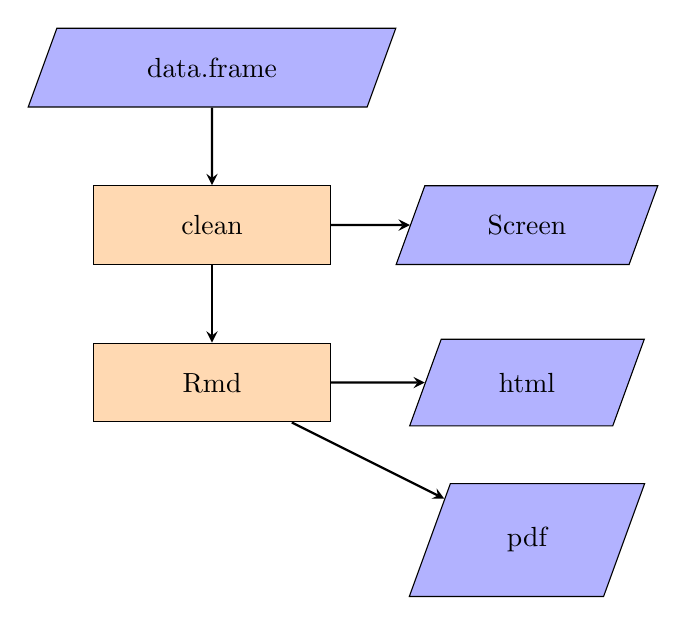
\begin{tikzpicture}[node distance=2cm]
\node (start) [io] {data.frame};
\node (pro1) [process, below of=start] {clean};
\node (screen) [io, right of=pro1, xshift=2cm] {Screen};
\node (pro2) [process, below of=pro1] {Rmd};
\node (html) [io, right of=pro2, xshift=2cm] {html};
\node (pdf) [io, below of=html] {pdf};
\draw [arrow] (start) -- (pro1);
\draw [arrow] (pro1) -- (screen);
\draw [arrow] (pro1) -- (pro2);
\draw [arrow] (pro2) -- (html);
\draw [arrow] (pro2) -- (pdf);
\end{tikzpicture}
\end{center}
\label{fig:flowchart1}
\caption{The process of cleaning data frames using the \pkg{cleanR}
  package. A series of check is applied to each variable in a
  \texttt{data.frame} and a summary of the result is either printed to
  the screen, or an \proglang{R} markdown file is produced which is
  subsequently rendered.}
\end{figure}

\section{Checking a dataset for errors} \label{sec:example1}

In \pkg{cleanR} the clean function

\begin{Schunk}
\begin{Sinput}
> library(cleanR)
> data(testData)
> head(testData)
\end{Sinput}
\begin{Soutput}
  charVar factorVar numVar intVar boolVar keyVar emptyVar _joeVar jack__var
1       a         a      1      1    TRUE      1        1       1         1
2       b         b      2      2   FALSE      2        1       2         2
3       c         c      3      3    TRUE      3        1       3         3
4       a         a      4      4    TRUE      4        1       4         4
5       b         b      5      5    TRUE      5        1       5         5
6       d         d      6      6   FALSE      6        1       6         6
  numOutlierVar smartNumVar      cprVar   cprKeyVar miscodedMissingVar
1             1           0 010101-1111 010101-1111                  .
2             2           0 020102-2929 020102-2929                   
3             3           0 121201-1902 121201-1902                nan
4             4           0 030729-2222 030729-2222                NaN
5             5           0 080909-1212 080909-1212                NAN
6             6           0 010101-1111 020202-0101                 na
\end{Soutput}
\end{Schunk}


\begin{Schunk}
\begin{Sinput}
>                                         # clean(testData)
> 2+3
\end{Sinput}
\begin{Soutput}
[1] 5
\end{Soutput}
\end{Schunk}


% \includepdf[fitpaper=true, pages=-]{test.pdf}

Arguments

\section{The structure of \pkg{cleanR}} \label{sec:internals}

asd
asd


\section{Extending \pkg{cleanR} by adding custom error checks} \label{sec:extending}

Lav en situation svarende til eksemplet

\begin{Schunk}
\begin{Sinput}
> characterFoo <- function(v) {
+     if (substr(substitute(v), 1, 1) == "_") {
+         out <- list(problem=TRUE, message="Note that the variable name begins with \\_")
+     } else out <- list(problem=FALSE, message="")
+     out
+ }
> class(characterFoo) <- "checkFunction"
> attr(characterFoo, "description") <- "I really hate underscores"
> #clean(testData, characterChecks=c(defaultCharacterChecks(), "characterFoo"))
> 
\end{Sinput}
\end{Schunk}


Lav også et eksempel med rangecheck.




\section{Using the online web-app} \label{sec:web-app}

asd
asd

\end{document}
